\documentclass{beamer}

\usetheme{Warsaw}

\usepackage[T1,T2A]{fontenc}
\usepackage[utf8]{inputenc}
\usepackage[english,russian]{babel}
\usepackage{amssymb,amsfonts,amsmath,mathtext,float}  

\makeatletter
\renewcommand{\@biblabel}[1]{#1.} % Заменяем библиографию с квадратных скобок на точку:
\makeatother

\usepackage{csquotes}

%\usepackage{bibunits}  
\setbeamertemplate{bibliography item}[text]
%\defaultbibliography{plain}
%\defaultbibliographystyle{IEEEtran}

\usepackage{caption}
\DeclareCaptionLabelSeparator{par}{\par}
\newcommand\tablecaption[1]{
	\captionsetup{labelsep=par,justification=raggedleft}
	\caption{#1}
}

\usepackage{bm}

\usepackage{multirow}

\usepackage{rotating}

\usepackage[noend]{algorithmic}
\usepackage{algorithm}

\newcommand{\algname}[1]{\textsc{#1}}

\renewcommand{\algorithmicrequire}{\textbf{Input:}}
\renewcommand{\algorithmicensure}{\textbf{Output:}}
\renewcommand{\algorithmicprint}{\textbf{output}}
\renewcommand{\algorithmiccomment}[1]{\hspace*{\fill}\{#1\}}

\algsetup{indent=2em}

\usepackage{amsthm}
\theoremstyle{definition}
%\newtheorem{definition}{Определение}

\addto\captionsrussian{\renewcommand{\bibname}{Список использованных источников}}


\def\cp#1{\preccurlyeq_{#1}}

\def\PP{\mathbb{P}}
\def\UCPP{\context^\PP_{\sim}}
\def\mpref{\leq}
\def\cprime{^{\sim}}

\def\ABC{A \cp{C} B}
\def\DEF{D \cp{F} E}

\def\minivan{\textrm{minivan}}
\def\suv{\textrm{SUV}}
\def\red{\textrm{red}}
\def\white{\textrm{white}}
\def\bright{\textrm{bright}}
\def\price{\textrm{price}}
\def\dark{\textrm{dark}}

\def\Z{\mathcal{Z}}

\makeatletter
\def\@makechapterhead#1{%
	\vspace*{50\p@}%
	{\parindent \z@ \raggedright \normalfont
		\interlinepenalty\@M
		\Huge\bfseries  \thechapter.\enskip #1\par\nobreak
		\vskip 40\p@
	}}
\makeatother
	

\makeatletter
\renewcommand{\ALG@name}{Алгоритм}
\renewcommand{\listalgorithmname}{Список алгоритмов}
\makeatother

%\usepackage[unicode]{hyperref}

\beamertemplatenavigationsymbolsempty
\setbeamertemplate{footline}[frame number]
\setbeamertemplate{itemize items}[default]
\setbeamertemplate{enumerate items}[default]

\title[Выявление предпочтений \enquote{при прочих равных}] % (optional, only for long titles)
{Экспериментальное исследование и модификация алгоритма выявления предпочтений \enquote{при прочих равных}}
\author[Садыков~Э.Р.]{Студент: Садыков~Эрнест~Рашидович, 401ПИ \\ 
	\vspace{1em}
	Научный руководитель: Объедков Сергей Александрович, к.т.н., доцент департамента анализа данных и искусственного интеллекта факультета компьютерных наук
}
\institute
{
	Национальный исследовательский университет\\
	Высшая школа экономики
}
\date{Москва, 2015}

\begin{document}
	\frame{\titlepage}
	\begin{frame}
		\frametitle{Актуальность проблемы}
		Применения рекомендательных алгоритмов:
		\begin{itemize}
			\item Интернет-магазины (amazon, ozon)
			\item Социальные сети (reddit, digg)
			\item Специализированные рекомендательные системы (last.fm, Имхонет)
		\end{itemize}
		
		\pause
		
		\vspace{1.5em}
		Рекомендации удерживают внимание пользователя на сайте

		\pause 
		
		\vspace{1.5em}
		В основе рекомендательных систем – алгоритмы выявления предпочтений
	\end{frame}
	
	\begin{frame}
		\frametitle{Цель и задачи}
		\emph{Цель}: реализовать и протестировать алгоритм обучения предпочтениям «при прочих равных» для проверки его применимости к реальным данным; разработать и протестировать модификации алгоритма, улучшающие его характеристики

		\pause
		\vspace{1em}
		
		\emph{Задачи}:
		\begin{itemize}
			\item Реализовать базовый алгоритм, описанный в \cite{Obiedkov:2013}
			\item Провести апробацию алгоритма на реальных данных 
			\item Провести сравнение работы базового алгоритма с другими методами машинного обучения
			\item Разработать модификации алгоритма, повышающие качество работы алгоритма
			\item Сравнить результаты работы модификаций алгоритма с другими методами машинного обучения
		\end{itemize}
	\end{frame}
	
	\begin{frame}
		\frametitle{Пример контекста}
		\begin{center}
		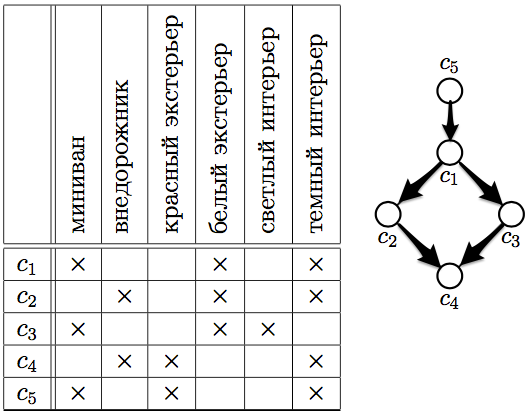
\includegraphics[width=80mm]{./images/context.png}
		\end{center}
		\vspace{-1.5ex}
		 $c_1, \dotsc, c_5$ – объекты (в данном случае автомобили) \\
		 ``миниван'', ``внедорожник'', \dots, ``темный интерьер'' – признаки \\
		 \vspace{1ex}
		 справа – граф предпочтений: $c_5$ предпочтительнее $c_1$; $c_2$ и $c_3$ несравнимы
	\end{frame}
	
	\begin{frame}
		Интуитивное описание метода 
	\end{frame}
	
	\begin{frame}
		\frametitle{Наборы данных}
		\begin{enumerate}
			\item \emph{Набор данных о предпочтениях в автомобилях}: 60 человек указывали свои предпочтения, выбирая из 10 автомобилей \cite{dataset:Abbasnejad:2013} \\
			\url{http://users.cecs.anu.edu.au/~u4940058/CarPreferences.html}
			\vspace{1em}
			\item \emph{Набор данных о предпочтениях в суши}: 5000 человек ранжировали 10 суши \cite{Kamishima:2003}
			\url{http://www.kamishima.net/sushi/}
		\end{enumerate}
	\end{frame}
	
	\begin{frame}
		%\frametitle{Проведение экспериментов}
		проведение экспериментов
	\end{frame}
	
	\begin{frame}
		\frametitle{Первый эксперимент}
		\framesubtitle{над базовой версией алгоритма}
		\begin{center}
			\begin{tabular}{|l|ll|}
				\hline
				Алгоритм             & 1-out & 2-out \\ \hline
				\enquote{при прочих равных}      & $59.09 \pm 3.08$ & $52.94 \pm 0.97$ \\
				C4.5                 & $79.91 \pm 7.29$ & $71.61 \pm 8.97$ \\
				Наивный байес. клас. & $83.76 \pm 7.2$ & $82.69 \pm 9.68$ \\ \hline
			\end{tabular}
		\end{center}
		
		\vspace{1.5em}
		Алгоритм выявления предпочтений \enquote{при прочих равных} для большинства пар $(x,y)$ находит аргументы и за $x \leq y$, и за $y \leq x$.
	\end{frame}
	
	\begin{frame}
		\frametitle{Пример}
		\begin{center}
			Сравним два автомобиля:
		\end{center}
		\begin{columns}[c] 
			\column{.5\textwidth} 
			Красный внедорожник с темным интерьером
	    	\column{.5\textwidth}
	    	Красный миниван со светлым интерьером
		\end{columns}
		\begin{center}
			\vspace{2em}
			\emph{лучше} потому что \\внедорожники лучше миниванов \\
			\vspace{2em}
			\emph{хуже} потому что \\темный интерьер хуже светлого 
		\end{center}
	\end{frame}
	
	\begin{frame}
		\frametitle{Модификация 1}
		\framesubtitle{подсчет ``подтверждающих'' пар объектов}
		Считаем количество пар объектов обучающей выборки, которые ``подтверждают'' предпочтение. 
		\vspace{1.4em}
		\begin{columns}[c] 
			\column{.5\textwidth} 
			Красный внедорожник с темным интерьером
			\column{.5\textwidth}
			Красный миниван со светлым интерьером
		\end{columns}
		\begin{center}
			\vspace{0.5em}
			\emph{лучше}: \\ 
			2 пары ``внедорожники лучше миниванов'' \\
			2 пары ``внедорожники лучше светлого интерьера при одинаковом экстерьере'' \\
			\vspace{1em}
			\emph{хуже}: \\
			3 пары ``темный интерьер хуже светлого''
		\end{center}
		
		\vspace{1.5em}
		Таким образом, красный внедорожник с темным интерьером {\color{green} лучше} красного минивана со светлым интерьером (4 против 3).
	\end{frame}
	
	\begin{frame}
		\frametitle{Модификация 2}
		\framesubtitle{поиск наиболе ``сильных'' предпочтений}
		Ищем такое предпочтение, которое подкреплено максимальным количеством ``подтверждающих'' пар.
		\vspace{1.4em}
		\begin{columns}[c] 
			\column{.5\textwidth} 
			Красный внедорожник с темным интерьером
			\column{.5\textwidth}
			Красный миниван со светлым интерьером
		\end{columns}
		\begin{center}
			\vspace{0.5em}
			\emph{лучше}: \\ 
			2 пары ``внедорожники лучше миниванов'' \\
			2 пары ``внедорожники лучше светлого интерьера при одинаковом экстерьере'' \\
			\vspace{1em}
			\emph{хуже}: \\
			3 пары ``темный интерьер хуже светлого''
		\end{center}
		
		\vspace{1.5em}
		Таким образом, красный внедорожник с темным интерьером {\color{red} хуже} красного минивана со светлым интерьером (2 против 3).
	\end{frame}
	
	\begin{frame}
		Модификация: бинарные отношения	
	\end{frame}
	
	
	\begin{frame}
		\frametitle{Результаты}
		\begin{itemize}
			\item Реализован базовый алгоритм выявления предпочтений «при прочих равных»
			\item Проведена апробация алгоритма на двух реальных наборах данных: cars dataset \cite{dataset:Abbasnejad:2013}, sushi dataset \cite{Kamishima:2003} 
			\item Проведено сравнение работы базового алгоритма с другими методами машинного обучения
			\item Разработано 3 модификации алгоритма, повышающие качество работы базового алгоритма (подумать)
			\item Экспериментально обоснована состоятельность подхода, лежащего в основе базовой версии алгоритма и показана  эффективность его (алгоритма) модификаций
		\end{itemize}
		\pause
		\begin{itemize}
			\item {\color{gray} Написан инструментарий для сравнения алгоритмов: классы для проведения экспериментов, утилита с GUI для запуска экспериментов}
		\end{itemize}
	\end{frame}
		
	\begin{frame}[plain,c]
		\begin{center}
			\Huge Спасибо за внимание!
		\end{center}
	\end{frame}

	\begin{frame}[allowframebreaks]
		\frametitle{Список использованных источников}
		\bibliographystyle{apalike}
		\bibliography{bibliography}
	\end{frame}
	
	%%\setcounter{page}{2}
	%\tableofcontents 
	%\chapter*{Реферат}
\addcontentsline{toc}{chapter}{Реферат}

Работа состоит из \pageref{LastPage} страниц, 3 глав, содержит 2 таблицы и 1 иллюстрацию. 

\vspace{2em}

Задача ранжирования одна из наиболее активно развиваемых областей обучения предпочтениям. В этой работе представлена реализация алгоритма выявления предпочтений при прочих равных. Этот алгоритм работает с попарными предпочтениями, а значит для его использования не требуется выявления функции полезности. В работе представлено эмпирическое исследование реализации, основанной на формальном определении алгоритма. Количественные показатели результатов экспериментов, проведенных над алгоритмом, сравниваются с другими методами машинного обучения. Так же в работе представлена модификация, расширяющая область применения алгоритма. Проведенные эксперименты показали, что алгоритм адекватно работает на реальных наборах данных.

\textbf{Ключевые слова}: обучение предпочтениям, машинное обучение, предпочтения при прочих равных, обучение ранжированию, попарные предпочтения 


\vspace{2em}


Ranking problem is one of the most extensively studied field of preference learning. In this paper an implementation of the ceteris paribus preference elicitation algorithm is presented. This algorithm works with binary relations and supports purely relative data that has no utility function. Based on the formal description of the algorithm, we conduct an empirical study of its implementation. To quantitative measurement of the implementation is compared with various machine learning techniques. In addition, we propose a modification of the algorithm, which expand its scope. Results of conducted experiments proves the ability of the algorithm to work with real-world datasets.

\textbf{Keywords}: preference learning, machine learning, ceteris paribus preferences, learning to rank, pair preferences
	%%\chapter*{Определения, сокращения и обозначения}
\addcontentsline{toc}{chapter}{Определения, сокращения и обозначения}
	%\chapter*{Введение}
\addcontentsline{toc}{chapter}{Введение}

Обучение предпочтениям (preference learning) – одна из наиболее развиваемых областей машинного обучения. Главная задача алгоритмов выявления предпочтений – конструирование модели, основанной на тренировочном наборе данных, и предсказание отношений предпочтений в случае добавления новых объектов в модель.

В настоящее время исследователи наибольшее внимание уделяют задачи ранжирования. У обучения ранжированию существует большое количество приложений. Например, розничные сети могут предсказывать предпочтения клиента, основываясь на его демографических данных, таких как пол, возраст, семейное положение и т.п. Другим примером является биоинформатика, где для упорядочивания генов применяется ранжирование, основанное на филогенетических данных. \cite{Balasubramaniyan:2005} Поисковые движки используют алгоритмы ранжирования для упорядочивания поисковой выдачи. Более того, обучение ранжированию может быть использовано для упорядочивания самих алгоритмов ранжирования\cite{Brazdil:2003}.

Основная часть данной работы посвящена различным алгоритмам выявления предпочтений. Задача таких алгоритмов заключается в ранжировании множества объектов. Обычно алгоритмы выявления предпочтений являются одним из ключевых модулей рекомендательных систем. Такие системы пытаются \enquote{угадать} предпочтение пользователя, используя информацию о его предыдущих действиях и действиях пользователей, похожих на него. Примерами таких систем являются сервисы imhonet.ru\footnote{http://imhonet.ru/about/ – о проекте Имхонет}, kinopoisk.ru\footnote{http://www.kinopoisk.ru/docs/join/ - о возможностях Кинопоиска}, last.fm\footnote{http://www.lastfm.ru/about – о проекте last.fm} и многие другие.

Основная \emph{цель} данной работы – исследование алгоритма выявления предпочтений \enquote{при прочих равных} (далее - Алгоритм), который был описан в \cite{Obiedkov:2013}. Основные \emph{задачи}:
\begin{enumerate} 
	\item Реализация Алгоритма на одном из прикладных языков программирования
	\item Сравнение результатов работы Алгоритма с другими алгоритмами обучения предпочтений и классическими методы машинного обучения
	\item Модификация Алгоритма, заключающаяся в расширении его области действия и повышения его производительности
\end{enumerate}

\section*{Структура работы}
В Главе \ref{chapter:literature} представлен литературный обзор. В Главе \ref{chapter:theory} представлен необходимый теоретический базис, дана классификация задач ранжирования, а так же описан Алгоритм и показан пример его работы.
%Глава \ref{chapter:experiments} посвящена экспериментальным данным: в ней описана методика исследования Алгоритма, а так же полученные результаты.
	%\chapter{Обзор существующих решений}
\label{chapter:literature}

На тему задач ранжирования написано множество литературы. Помимо отдельных статьей опубликовано несколько сборников, посвященных данной проблеме. Примером такого сборника является \textit{Preference Learning} \cite{plbook:2010} Фюрнкранца и Хюллермайера (F{\"{u}}rnkranz \& H{\"{u}}llermeier), в котором авторы собрали широкий спектр различных работ на тему обучения предпочтений. Лиу (Liu) в \textit{Learning to Rank for Information Retrieval} \cite{Liu:2011} представил обширные исследования задач ранжирования. Однако, основное внимание Лиу уделяет задачам извлечение информации, в то время как данная работа посвящена упорядочиванию объектов.

Фюрнкранц и Хюллермайер в \cite{plbook:Introduction:2010} представляют подробную классификацию задач ранжирования и методов для их решения. Подробнее данная классификация описана в Главе \ref{chapter:theory}. В другой работе \cite{Furnkranz:2003} авторы описывают алгоритм ранжирования, который выводит функцию полезности на основе отношений предпочтения.

Было предложено несколько методов для создания модели предпочтений. Хэддави (Haddawy et al.) \cite{Haddawy:2003} описал метод выявления предпочтений, основанный на простой нейросети. Жадный алгоритм, находящий аппроксимацию задачи ранжирования представил Кохен (Cohen) в \cite{Cohen:1999}.

Целый ряд алгоритмов машинного обучения был адаптирован для задач ранжирования. Примером такой адаптации является исследование, проведенное Женгом (Zheng et al.) \cite{Zheng:2007}, где был предложен метод сведения задачи ранжирования к задачи регрессии. В дополнение, Бургерс (Burges et al.) \cite{Burges:2005} описал подход к задачи ранжирования, основанный на алгоритме градиентного спуска.

Камишима (Kamishima) \cite{Kamishima:2003} описывает проведенное им исследование, которое доказывает несостоятельность применения семантического дифференциала \cite{Osgood:1957} к пользовательским предпочтениям. Данные, собранные автором, показывают, что оценка альтернатив с помощью числовой шкалы не совпадает с более интуитивным методом сбора предпочтений – ранжированием. Отметим, что ранжированный список предпочтений и попарные предпочтения, рассматриваемые в настоящей работе, могут быть тривиальным образом трансформированы друг в друга.

%TODO: указать какие задачи еще существуют
Хотя существует множество задач в сфере выявления предпочтений, в данной работе мы рассматриваем проблему ранжирования. Данная глава посвящена теоретическим основам задачи упорядочивания. Большая часть материала данной главы основана на \enquote{Введении} из сборника \textit{Preference Learning} Фюрнкранца и Хюллермайера\cite{plbook:Introduction:2010}.

Остальная часть данной главы организована следующим образом: в первом разделе описан теоретический базис задач ранжирования, во втором представлены уже существующие алгоритмы, которые участвуют в экспериментах в Главе~\ref{chapter:experiments}.

\section{Теоретические основы задач ранжирования}

	Алгоритмы ранжирования могут отличаться друг от друга по ряду признаков. Так, часть алгоритмов работают с линейно упорядоченными множествами (полным порядком), в то время как другие работают с частичным порядком. Говорят, что отношение предпочтения является полным порядком, если любые две альтернативы связаны отношением предпочтения. Это значит, что из каждой пары объектов\footnote{В данной работе слово \enquote{объект} используется как термин анализа формальных понятий. Подробнее см. раздел \ref{subsection:definitions}} можно однозначно выбрать более предпочитаемый вариант (или, по крайней мере, выбрать вариант не хуже). С другой стороны, частичный порядок допускает существование пар объектов, которые не связаны между собой отношением предпочтения. 
	\begin{definition}
		\label{def:total_order}
		Отношение порядка $\leq$, для которого выполняется условие
		$\forall x,y\in X \quad  x\leq y \vee y \leq x$,
		называется \emph{полным порядком}.
	\end{definition}
	
	Предпочтения могут находиться в различных отношениях: предпорядка (preorder), нестрого порядка (nonstrict order) или строгого порядка (strict order). Так, строгое отношение между объектами $a$ и $b$ может быть интерпретировано как \enquote{$a$ лучше $b$}, в то время как нестрогие отношения означают утверждения вида \enquote{$a$ не хуже $b$}\cite[с.~384]{Barten:1982}. Предпорядок – это нестрогий порядок без свойства антисимметричности. Определения \ref{def:preorder}, \ref{def:nonstrict_order} и \ref{def:strict_order} представляют формальные описания данных понятий.
	
	\begin{definition}
		\label{def:preorder}
		Отношение $\leq$ называется \emph{предпорядком} (или квазипорядком) на множестве $S$, если оно удовлетворяет следующим условиям\cite{harel:2000}:
		\begin{itemize}[itemsep=-1.5mm]
			\item Рефлексивность: $a \leq a \quad \forall a \in S$
			\item Транзитивность: $a \leq b\: \wedge\: b \leq c \implies a \leq c$ 
		\end{itemize}
	\end{definition}	
	\begin{definition}
		\label{def:nonstrict_order}
		Множество $S$ находится в \emph{нестрогом порядке}, если это множество – предпорядок, и на нем выполняется свойство антисимметричности\cite{Skiena:1991}: $a \leq b\; \wedge\; b \leq a \implies a = b$.
	\end{definition}
	\begin{definition}
		\label{def:strict_order}
		Множество $S$ находится в \emph{строгом порядке}, если на этом множестве выполняются следующие свойства:
		\begin{itemize}[itemsep=-1.5mm]
			\item Антирефлексивность: $ a \nless a \quad \forall a \in S$
			\item Асимметричность: $a < b \implies b \nless a \quad \forall \, (a, b) \in S$
			\item Транзитивность: $a < b\: \wedge\: b < c \implies a < c$
		\end{itemize}
		Если в нестрогом порядке условие рефлексивности заменить на антирефлексивность, получится строгий порядок.
	\end{definition}
	
	Алгоритм выявления предпочтений \enquote{при прочих равных} работает с предпорядками.
	
	\subsection{Типы задач ранжирования}
	Фюрнкранц и Хюллермайер в \cite{plbook:Introduction:2010} выделяют три типа задач ранжирования: ``ранжирование меток" (\emph{label ranking}), ``ранжирование экземпляров'' (\emph{instance ranking}) и ``ранжирование объектов'' (\emph{object ranking}).
	
	\subsubsection{Ранжирование меток}
	Данный тип ранжирования используется в ситуациях, когда надо найти порядок фиксированного набора элементов в зависимости от предоставленного контекста. Примером такого ранжирования может является упорядочение списка товаров в зависимости от личных данных клиента.
	
	\begin{figure}[h!]
		\hrule
		\begin{description}[nosep]
			\item[Дано:] \null\leavevmode
			\begin{itemize}[itemsep=0pt,leftmargin=2ex,label=\textbf{---}]
				\item обучающий набор данных $\{\bm{x}_\ell \, | \, \ell = 1,2,\dotsc,n\} \subseteq \mathcal{X} $ (обычно, но не обязательно, каждый экземпляр представлен в виде вектора атрибутов)
				\item множество меток $\mathcal{Y} = \{y_i\,|\,i = 1,2,\dotsc,k\}$
				\item для каждого экземпляра тренировочного набора данных $\bm{x}_\ell$: множество попарных предпочтений в виде $y_i \succ_{\bm{x}_\ell} y_j $ (данная нотация читается как ``для данного $\bm{x}_\ell$  метка $y_i$ предпочитается метке $y_j$'')
			\end{itemize}
			\item[Найти:] \null\leavevmode
			\begin{itemize}[itemsep=0pt,leftmargin=2ex,label=\textbf{---}]
				\item функцию ранжирования, которая отображает каждый $\bm{x} \in \mathcal{X}$ в перестановку $\succ_{\bm{x}_\ell}$ множества $\mathcal{Y}$
			\end{itemize}
		\end{description} 
		\hrule
		\label{fig:label_ranking}
	\end{figure}
	
	%TODO: переформулировать
	\subsubsection{Ранжирование экземпляров}
	Данный тип используется в случаях, когда необходимо каждый из объектов отнести к одному из классов из фиксированного набора. Такое ранжирование обычно используется для оценки альтернатив, таких как оценка фильма в рекомендательной системе.
	
	\begin{figure}[h!]
		\hrule
		\begin{description}[nosep]
			\item[Дано:] \null\leavevmode
			\begin{itemize}[itemsep=0pt,leftmargin=2ex,label=\textbf{---}]
				\item набор тренировочных данных $\{\bm{x}_\ell \, | \, \ell = 1,2,\dots,n\} \subseteq \mathcal{X} $ (обычно, но не обязательно, каждый экземпляр представлен в виде вектора атрибутов)
				\item множество меток $\mathcal{Y} = \{y_i\,|\,i = 1,2,\dotsc,k\}$ и их порядок $y_1 < y_2 < \dotsb < y_k$ 
				\item соответствие каждого экземпляра тренировочного набора данных $\bm{x}_\ell$ метке $y_\ell$
			\end{itemize}
			\item[Найти:] \null\leavevmode
			\begin{itemize}[itemsep=0pt,leftmargin=2ex,label=\textbf{---}]
				\item функцию, которая позволяет ранжировать множество экземпляров $\{\bm{x}_j\}^t_{j=1}$ согласно (неизвестному) уровню предпочтений
			\end{itemize}
		\end{description} 
		\hrule
		\label{fig:instance_ranking}
	\end{figure}
	
	\subsubsection{Объектное ранжирование}
	Алгоритмы для объектного ранжирования работают с 
	относительной %TODO: использовать другое слово
	информацией, в которой отсутствуют предопределенные категории. Для данной работы это наиболее важный тип ранжирования, так как  Алгоритм работает именно с попарными отношениями объектов (относительный порядок). Пример данного типа ранжирования приведен в разделе \ref{subsection:example}.
	
	Ниже представлено формальное определение объектного ранжирования. Алгоритм выявления предпочтений \enquote{при прочих равных} решает более узкую задачу: на вход приходит множество уже проранжированных объектов $\Z \setminus \{e\}$ и объект $e$. Работа алгоритма заключается в упорядочении множества $\Z$.
	
	\begin{figure}[h!]
		\hrule
		\begin{description}[nosep]
			\item[Дано:] \null\leavevmode
			\begin{itemize}[itemsep=0pt,leftmargin=2ex,label=\textbf{---}]
				\item множество (возможно, бесконечное) объектов $\Z$ (обычно, но не обязательно, каждый объект представлен в виде вектора признаков)
				\item конечное множество попарных предпочтений $\bm{x}_i \succ \bm{x}_j, \: (\bm{x}_i, \bm{x}_j) \in \Z \times \Z$
			\end{itemize}
			\item[Найти:] \null\leavevmode
			\begin{itemize}[itemsep=0pt,leftmargin=2ex,label=\textbf{---}]
				\item функцию ранжирования $f(\cdot)$, которая принимает на вход множество объектов и возвращает перестановку (ранжирует) этого множества
			\end{itemize}
		\end{description} 
		\hrule
		\label{fig:object_ranking}
	\end{figure}
	
	\subsection{Подходы к реализации}
	В \cite{plbook:Introduction:2010} представлено четыре подхода к реализации алгоритмов ранжирования. 
	Первый вариант – выявить \emph{функцию полезности} (learning utility function) и построить полный порядок, основываясь на значениях, полученных с помощью этой функции. Такой подход применим ко всем трем типам задач ранжирования. 
	Второй подход заключается в \emph{выявлении зависимостей} в попарных отношениях предпочтения (learning preference relations). Хотя часто подобный способ и создает более простую модель, в некоторых случаях может возникать нарушение транзитивности\cite[с.~10]{plbook:Introduction:2010}. 
	Третий подход называется \emph{обучение предпочтениям, основанное на модели} (model-based preference learning). Он используется в случаях, когда известны некоторые ограничения об отношениях предпочтения. 
	Последний подход, который выделяют авторы, называется \emph{локальное агрегирование предпочтений} (local aggregation of preferences). Основная идея данного метода заключается в поиске ближайших \enquote{соседей} для данного объекта.
	
	Очевидно, что описанные подходы не являются взаимоисключающими. Алгоритм выявления предпочтений \enquote{при прочих равных} является примером смешения подходов: с одной стороны, Алгоритм имеет дело с бинарными отношениями и подходит к типу ``выявления зависимостей''; с другой стороны, он работает с отношениями \enquote{при прочих равных}, что накладывает определенные ограничения на результирующую модель. Следовательно, Алгоритм так же может быть отнесен к обучению, ``основанному на модели''.

\section{Рассматриваемые алгоритмы}

	Как описано в Введении, первоочередная задача данной работы – сравнение Алгоритма \ref{algo:prediction} с другими методами машинного обучения. В сравнении участвуют методы классифицирующих деревьев, а так же Байесовские методы. В разделах \ref{subsec:c4.5} -- \ref{subsec:bayes_net} подробно описаны эти алгоритмы.
	
	\subsection{C4.5}
	\label{subsec:c4.5}
		Алгоритм C4.5 был впервые представлен Квинланом (Quinlan) в \cite{Quinlan:1993} в 1993 году, и с тех пор стал одним из самых популярных реализаций деревьев принятия решений. С4.5 является расширением алгоритма ID3 \cite{Quinlan:1986}, так же разработанным Квинланом в 1968 году. Оба этих алгоритма основаны на расчете информационной энтропии. 
		
		C4.5 предназначен для построение классифицирующих деревьев. Имея значения признаков обучающей выборки, алгоритм на каждом шаге производит ветвление по признаку, которые дает максимальный прирост информации. По сравнению с ID3, C4.5 производит ряд оптимизаций, таких как отсечение ветвей (pruning). Кроме того, в C4.5 была добавлена поддержка числовых признаков.
	
	\subsection{Наивный Байесовский классификатор}
	\label{subsec:naive_bayes}
		Наивный Байесовский классификатор – это простой статистический классификатор, основанный на применении теоремы Байеса с предусловием независимости признаков. Первые упоминания практического применения теоремы Байеса относятся к 18 веку. \cite{Stigler:1983}
	
	\subsection{Байесовская сеть}
	\label{subsec:bayes_net}
		Байесовская сеть является графом, в вершинах которого находятся переменные, а дуги выражают зависимость между этими переменными. Таким образом, сеть выражает отношения между переменными, что позволяет строить классификаторы на ее основе. Данный подход к классификации был формализован Перлом (Pearl) в \cite{Pearl:1985}. В данной работе используется реализация Байесовской сети из фреймворка Weka \cite[с.~111-123]{WekaManual}.
	%\chapter{Теоретические основы}
\label{chapter:theory}

%TODO: указать какие задачи еще существуют
Хотя существует множество задач в сфере выявления предпочтений, в данной работе мы рассматриваем проблему ранжирования. Данная глава посвящена теоретическим основам задачи упорядочивания. Тем не менее, от читателя ожидается знание основ теории множеств. Большая часть материала данной главы основана на \enquote{Введении} из сборника \textit{Preference Learning} Фюрнкранца и Хюллермайера\cite{plbook:Introduction:2010}.


\section{Теоретические основы задач ранжирования}

	Алгоритмы ранжирования могут отличаться друг от друга по ряду признаков. Так, часть алгоритмов работают с линейно упорядоченными множествами (полным порядком), в то время как другие работают с частичным порядком. Говорят, что отношение предпочтения является полным порядком, если про любые две альтернативы соединены отношением предпочтения. Это значит, что из каждой пары объектов\footnote{В данной работе слово \enquote{объект} используется как термин анализа формальных понятий. Подробнее см. секцию \ref{subsection:definitions}} можно однозначно выбрать более предпочитаемый вариант (или, по крайней мере, выбрать вариант не хуже). С другой стороны, в случае частичного порядка могут существовать пары объектов, которые не связаны между собой отношением предпочтения.
	%TODO: формальное описание полного и частичного порядков
	
	Предпочтения могут находиться в различных отношениях: предпорядка (preorder), нестрого порядка (partial order) или строгого порядка (strict order). Так, строгое отношение между объектами $a$ и $b$ может быть интерпретировано как \enquote{$a$ лучше $b$}, в то время как нестрогие отношения означают утверждения вида \enquote{$a$ не хуже $b$}\cite[p.~384]{Barten:1982}. Предпорядок – это нестрогий порядок без свойства антисимметричности. Определения \ref{def:preorder}, \ref{def:partial_order} и \ref{def:strict_order} дают более формальные описания данных понятий.
	
	\begin{definition}
	\label{def:preorder}
		Отношение $\leq$ называется \emph{предпорядком} (или квазипорялком) на множестве $S$, если оно удовлетворяет следующим условиям\cite{harel:2000}:
		\begin{itemize} 
			\item Рефлексивность: $a \leq a \quad \forall a \in S$
			\item Транзитивность: $a \leq b\; \textrm{and}\; b \leq c  \implies a \leq c$ 
		\end{itemize}
	\end{definition}	
	\begin{definition}
	\label{def:partial_order}
		Множество $S$ находится в \emph{нестрогом порядке}, если на это множество – предпорядок, и на нем выполняется свойство антисимметричности\cite{Skiena:1991}: $a \leq b\; \textrm{and}\; b \leq a \implies a = b$.
	\end{definition}
	\begin{definition}
	\label{def:strict_order}
		Множество $S$ находится в \emph{строгом порядке}, если на этом множестве выполняются следующие свойства\cite{???}:
		\begin{itemize}
			\item Антирефлексивность: $ a \nless a \quad \forall a \in S$
			\item Асимметричность: $a < b \implies b \nless a \quad \forall \, (a, b) \in S$
			\item Транзитивность: $a < b\; \textrm{and}\; b < c \implies a < c$
		\end{itemize}
		Если в нестрогом порядке условие рефлексивности заменить на антирефлексивность, получится строгий порядок.
	\end{definition}

	
	Так же алгоритмы могут быть разделены по признаку возможности работы с нестрогими отношениями. Так, строгое отношение между объектами $a$ и $b$ может быть интерпретировано как \enquote{$a$ лучше $b$}, в то время как нестрогие отношения означают утверждения вида \enquote{$a$ не хуже $b$}.\cite[p.~384]{Barten:1982} Алгоритм выявления предпочтений \enquote{при прочих равных} может работать только с частичным порядком и нестрогим отношением предпочтения.

\subsection{Типы задач ранжирования}
	Фюрнкранц и Хюллермайер в \cite{plbook:Introduction:2010} выделяют три типа задач ранжирования: ``ранжирование меток" (\emph{label ranking}), ``ранжирование экземпляров'' (\emph{instance ranking}) и ``ранжирование объектов'' (\emph{object ranking}).
	
	\subsubsection{Ранжирование меток}
		Данный тип ранжирования используется в ситуациях, когда надо найти порядок фиксированного набора элементов в зависимости от предоставленного контекста. Примером такого ранжирования может является упорядочение списка товаров в зависимости от личных данных клиента.
	
	%TODO: переформулировать
	\subsubsection{Ранжирование экземпляров}
		Данный тип используется в случаях, когда необходимо каждый из объектов отнести к одному из классов из фиксированного набора. Такое ранжирование обычно используется для оценки альтернатив, таких как оценка фильма в рекомендательной системе.
	
	\subsubsection{Объектное ранжирование}
		Алгоритмы для объектного ранжирования работают с 
		относительной %TODO: использовать другое слово
		информацией, в которой отсутствуют предопределенные категории. Для данной работы это наиболее важный тип ранжирования, так как рассматриваемый нами Алгоритм работает именно с попарными отношениями объектов (относительный порядок). Пример данного типа ранжирования приведен в секции \ref{subsection:example}.
		
		Так как в данной работе наиболее часто применение находит именно объектное ранжирование, на рис. \ref{fig:object_ranking} дано его формальное определение. Алгоритм выявления предпочтений \enquote{при прочих равных} решает более узкую задачу: на вход приходит множество уже проранжированных объектов $\Z \setminus \{e\}$ и объект $e$. Работа алгоритма заключается в упорядочении множества $\Z$.
		
		\begin{figure}[h]
			\hrule
			\begin{description}[nosep]
				\item[Дано:] \null\leavevmode
				\begin{itemize}[itemsep=0pt,leftmargin=2ex,label=\textbf{---}]
					\item множество (возможно, бесконечное) объектов $\Z$ (обычно (но не обязательно) каждый объект представлен в виде вектора атрибутов)
					\item конечное множество попарных предпочтений $x_i \succ x_j, (x_i, x_j) \in \Z \times \Z$
				\end{itemize}
				\item[Найти:] \null\leavevmode
				\begin{itemize}[itemsep=0pt,leftmargin=2ex,label=\textbf{---}]
					\item функцию ранжирования $f(\cdot)$, которая принимает на вход множество объектов и возвращает перестановку (ранжирует) этого множества
				\end{itemize}
			\end{description} 
			\hrule
			\caption{\it Определение объектного ранжирования (определение из \cite[Рис.~3]{plbook:Introduction:2010})}
			\label{fig:object_ranking}
		\end{figure}
	
	\subsection{Подходы к реализации}
		В \cite{plbook:Introduction:2010} представлено четыре подхода к реализации алгоритмов ранжирования. 
		Первый вариант – найти \emph{функцию полезности} и построить полный порядок основываясь на значениях, полученных с помощью этой функции. Такой подход применим ко всем трем типам задач ранжирования. 
		Второй подход заключается в \emph{выявлении зависимостей} в попарных отношениях предпочтения. Хотя часто подобный способ и создает более простую модель, в некоторых случаях может возникать нарушение транзитивности\cite[стр.~10]{plbook:Introduction:2010}. 
		Третий подход называется \emph{обучение предпочтениям, основанное на модели} и используется в случаях, когда известны некоторые ограничения об отношениях предпочтения. 
		Последний подход, который выделяют авторы, называется \emph{локальное агрегирование предпочтений}. Основная идея данного метода заключается в поиске ближайших \enquote{соседей} для данного объекта.
		
		Очевидно, что описанные подходы не являются взаимоисключающими. Алгоритм выявления предпочтений \enquote{при прочих равных} является примером смешения подходов. С одной стороны, Алгоритм имеет дело с бинарными отношениями и подходит к типу ''выявления зависимостей''. С другой стороны, он работает с отношениями \enquote{при прочих равных}, что накладывает определенные ограничения на результирующую модель. Следовательно, Алгоритм так же может быть отнесен к обучению, ''основанному на модели''.
	
	
\section{Алгоритм выявления предпочтений \enquote{при прочих равных}}

	Данный раздел основан на работе Объедкова \cite{Obiedkov:2013}, в которой представлен Алгоритм. Данный раздел состоит из двух секций: в первом представлен пример входных данных и описан ожидаемый результат работы Алгоритма, во втором представлено формальное определение Алгоритма.
	
	\subsection{Пример}
	\label{subsection:example}
		На рис. \ref{fig:pcxt} представлен пример контекста предпочтений. Объекты $c_1, \dots, c_5$ представляют машины, у каждой из которых есть свой набор признаков. Например, $c_2$ является белым внедорожником с темным интерьером. Диаграмма на правой стороне показывает отношение предпочтений какого-то пользователя: $c_1$ не хуже, чем $c_2$ и $c_3$; $c_5$ не хуже, чем $c_1$; $c_2$ и $c_3$ несравнимы; и так далее. 
		\begin{figure}
			\begin{center} 
				\cars \prefs
				\caption{\it Пример контекста предпочтений \cite[Рис.~1.1]{Obiedkov:2013}}
				\label{fig:pcxt}	
			\end{center} 
		\end{figure} 
		
		Задача алгоритма предсказать отношения предпочтения при добавлении нового объекта в контекст. В рассматриваемом примере в контекст может быть добавлен красный миниван с ярким интерьером, и Алгоритм должен выявить отношения предпочтения для добавленной машины, попарно сравнив её с $c_1, \dots, c_5$. 
	
	\subsection{Определения}
	\label{subsection:definitions}
		Представленный в данной работе алгоритм оперирует сущностями анализа формальных понятий\cite{Ganter:1999}, а так же понятиями, определенными в \cite{Obiedkov:2012:preferences,Obiedkov:2012:modeling}. В данном разделе представлены эти определения.
		
		
		\begin{definition}
			\emph{(Формальный) контекст} – это тройка $\context = (G, M, I)$, где $G$ называется множеством \emph{объектов}, $M$ называется множеством \emph{признаков}, и бинарное отношение ${I \subseteq G \times M}$ указывает на принадлежность признаков к каждому из объектов.
		\end{definition}
		
		Формаьлный контекст может быть визуализирован с помощью таблицы, такой как Рис. \ref{fig:pcxt}.
		
		Для множеств $A \subseteq G$ и $B \subseteq M$ следующим образом определены \emph{операторы Галуа} (derivation operators) $(\cdot)'$:
		\begin{center}
			$A'=\{m \in M \mid \forall g \in A (g I m)\}$
			
			$B'=\{g \in G \mid \forall m \in B (g I m)\}$
		\end{center}
		$A'$ – это набор признаков, которые есть у всех объектов множества $A$, а $B'$  –- набор объектов, каждый из которых содержит все признаки множества $B$. Пусть $g \in G$ и $m \in M$, тогда множества $\{g\}'$ и $\{m\}'$ называются \emph{содержание объекта} (object intent) и \emph{объем признака} (attribute extent), соответственно. Иногда их обозначают как $g'$ и $m'$.
		
		\begin{definition}
			\emph{Контекст предпочтений} $\PP = (G, M, I, \leq)$ это формальный контекст $(G, M, I)$ с рефлексивным и транзитивным отношением предпочтения $\leq$, определенным над $G$ (то есть, $\leq$ – предпорядок). Мы пишем $g < h$, если $g \leq h$ и $h \not\leq g$.
		\end{definition}
		
		Пример такого контекста представлен на Рис. \ref{fig:pcxt}.
		
		\begin{definition}
			Множество признаков $B \subseteq M$ \emph{предпочитается \enquote{при прочих равных}} множеству признаков $A \subseteq M$ по отношению ко множеству признаков $C \subseteq M$ в контексте предпочтений $\PP = (G, M, I, \leq)$ если 
			\[\forall g \in A' \forall h \in B'(\{g\}' \cap C = \{h\}' \cap C \to g \leq h).\]
			В таком случае мы говорим что предпочтение \emph{при прочих равных} $A \cp{C} B$ является \emph{валидным} или \emph{имеет место} в $\PP$ и обозначаем это как $\PP \models \ABC$.
		\end{definition}
	
	\subsection{Описание алгоритма}
		Чтобы найти предпочтение $\DEF$, поддерживаемое $\PP$, Алгоритм \ref{algo:prediction} итерируется по всем паром различных объектов $(g, h)$ контекста $\PP$ таких, что $g \leq h$. Для каждой такой пары он находит наиболее слабое предпочтение, которое объясняет и $g \leq h$, и предполагаемое предпочтение объекта, описываемого множеством признаков $B$, объекту, описываемого признаками $A$. Левая часть этого предпочтения должна согласовываться и с $g'$, и с $A$; таким образом, $D := A \cap g'$. Похожим образом определяется и правая часть: $E := B \cap h'$. Признаки в условии \enquote{при прочих равных} должны быть согласованы как с общей частью между $g$ и $h$, так и с общей часть между $A$ и $B$. Таким образом, $F$ является множеством, которое содержит все признаки, по которым нет расхождений между $g'$ и $h'$ и между $A$ и $B$: каждый признак из $F$ принадлежит и $g'$, и $h'$, или ни одному из них, аналогично с $A$ и $B$. %<..>
		Если после итерации по всем парам $g \leq h$ не удалось найти предпочтение $\DEF$, объясняющее почему $B$ должно предпочитаться $A$, значит таких предпочтений, поддерживаемых $\PP$, нет, и алгоритм отвечает отрицательно.
	
		\begin{algorithm}
			\caption{\algname{Предсказание предпочтения}$(A, B, \PP)$ \cite[Алг.~1]{Obiedkov:2013}}
			\label{algo:prediction}
			\begin{algorithmic}[1]
				\REQUIRE Содержания объектов $A, B \subseteq M$ и контекст предпочтений $\PP = (G, M, I, \leq)$.
				\ENSURE \TRUE, если $\PP$ поддерживает $\DEF$ для некоторого $D \subseteq A, E \subseteq B,$ и $F \subseteq M$ таких, что $F \cap A = F \cap B$; \FALSE, иначе.
				\item[]
				\FORALL{$g \in G$}
				\STATE $D := A \cap g'$
				\FORALL{$h \in G \setminus \{g\}$ таких, что $g \leq h$}
				\STATE $E := B \cap h'$
				\STATE $F := (M \setminus (A \vartriangle B)) \cap (M \setminus (g' \vartriangle h'))$
				\IF{$\PP \models \DEF$}
				\RETURN \TRUE
				\ENDIF
				\ENDFOR
				\ENDFOR
				\RETURN \FALSE
			\end{algorithmic}
		\end{algorithm}
		\begin{algorithm}
			\caption{\algname{Проверить предпочтение}$(\DEF, \PP)$ \cite[Алг.~2]{Obiedkov:2013}}
			\label{algo:check}
			\begin{algorithmic}
				\REQUIRE Предпочтение $\DEF$ над $M$ и контекст предпочтений $\PP = (G, M, I, \leq)$.%; assume that attribute extents, $m'$ for $m \in M$, are precomputed.
				\ENSURE \TRUE, если $\PP \models \DEF$; \FALSE, иначе.
				\STATE
				\STATE $X := \bigcap_{m \in D}m'$
				\STATE $Y := \bigcap_{m \in E}m'$
				\FORALL{$g \in X$}
				\FORALL{$h \in Y$}
				\IF {$g \not\leq h$ and $g' \cap {F} = h' \cap {F}$}
				\RETURN \FALSE
				\ENDIF
				\ENDFOR
				\ENDFOR
				\RETURN \TRUE
			\end{algorithmic}
		\end{algorithm}
		
	%\chapter{Эксперименты}
\label{chapter:experiments}
В данной главе представлена экспериментальная часть работы. Сравнение результатов работы алгоритма выявления предпочтений \enquote{при прочих равных} с другими методами обучения предпочтениям является ключевой частью данного исследования.

Глава состоит из трех разделов. В первом разделе представлены наборы данных, на которых сравнивались алгоритмы. Во втором описана методика сравнения алгоритмов и представлены результаты экспериментов. И в последней части кратко описаны инструменты, которые были использованы при проведении экспериментов.

\section{Входные данные}
	В данной работе
	апробация Алгоритма проводилась на двух наборах данных: набор данных о пользовательских предпочтениях в автомобилях и набор данных о предпочтениях в суши. Ниже подробно описан каждый из наборов данных.
	
	%TODO: перенести в секцию с описанием алгоритма
	%\subsection{Искусственный набор данных}
		%Искусственный набор взят из \cite{Obiedkov:2013}. Этот набор данных состоит из семи объектов, пять из которых представлены на рис.~\ref{fig:pcxt}. Еще два объекта: $c_6={minivan, red, bright}$ и $c_7={SUV, red, bright}$. Эти данные не много могут сказать о качестве работы алгоритма, но их можно использовать для базовой проверки его возможностей.
	
	\subsection{Набор данных об автомобильных предпочтениях}
	\label{subsec:cars_description}
		Первый реальный набор данных собран Аббаснеджадом и др. для \cite{dataset:Abbasnejad:2013}. Для сбора пользовательских предпочтений авторы использовали краудсорсинговую платформу Amazon Mechanical Turk\footnote{mturk.com – информация о проекте Amazon Mechanical Turk}. Набор данных состоит из двух экспериментов\footnote{Данные размещены по адресу: http://users.cecs.anu.edu.au/~u4940058/CarPreferences.html}: в первом была собрана информация от 60 пользователей о 10 машинах, во втором – от 60 пользователей о 20 машинах (далее – CD1 и CD2 обозначают первый и второй эксперимент, соответственно). Каждому из респондентов было предложено выбрать более предпочитаемый вариант из каждой пары автомобилей (всего 45 пар). Не все опрашиваемые ответили на полный список вопросов (для некоторых пользователей количество предпочтений менее 45). Причем в CD2 информации о каждой из машин было больше. Далее подробно описана информация, представленная в наборе данных.
		
		\vspace{1em}
		
		\noindent Характеристики пользователей:
		\vspace{-0.7em}
		\begin{itemize}[itemsep=-1.5mm]
			\item ID: уникальный идентификатор пользователя
			\item Образование: отсутствие ответа (0), старшая школа (1), бакалавриат (2), PhD (3)
			\item Возраст: отсутствие ответа (0), меньше 25 (1), от 25 до 30 (2), от 30 до 35 (3), больше 40 (4)
			\item Пол: отсутствие ответа (0), мужской (1), женский (2)
			\item Регион: отсутствие ответа (0), юг (1), запад (2), северо-восток (3), средний запад (4)
			\item Количество правильных ответов на контрольные вопросы: 3, 4 или 5
		\end{itemize}
		Данные собирались среди американской аудитории. Каждому пользователю было задано по пять контрольных вопросов, каждый из которых является одним из пользовательских предпочтений в обратном порядке (например, если пользователь указал, что $y < x$, то контрольный вопрос имеет вид $x < y?$, где $x$ и $y$ – какие-то объекты). На основе количества правильных ответов на контрольные вопросы можно судить о согласованности пользовательских предпочтений.
		
		\vspace{1em}
		
		\noindent Признаки машин:
		\vspace{-0.7em}
		\begin{enumerate}[itemsep=-1.5mm]
			\item Тип кузова: седан (1), SUV\footnote{SUV (англ. Sport Utility Vehicle или Suburban Utility Vehicle) – подобие внедорожника} (2), хэтчбек (3)
			\item Коробка передач: ручная (1), автоматическая (2)
			\item Объем двигателя: 2.5L, 3.5L, 4.5L, 5.5L, 6.2L
			\item Тип топлива: гибрид (1), не гибрид (2)
			\item Количество ведущих колес: все колеса ведущие (AWD, 4x4) (1), передние колеса ведущие (FWD) (2)
		\end{enumerate} 
		В первом эксперименте не были представлены хэтчбеки, а так же не использовалась информация о количестве ведущих колес.
	
	\subsection{Набор данных о предпочтениях в суши}
	\label{subsec:sushi_description}
		Набор данных собран Камишимой и Акахо и использован ими в \cite{Kamishima:2003}, \cite{Kamishima:2006} и других работах. Авторы опрашивали 5000 человек об их предпочтениях в суши (всего 100 наименований). При сборе данных авторы просили пользователей заполнить несколько опросников, в результате чего были сформированы 3 набора данных\footnote{Набор данных о предпочтениях суши доступен по адресу: http://www.kamishima.net/sushi/}:
		\begin{enumerate}[itemsep=-1.5mm]
			\item Выбрав 10 наиболее популярных суши, авторы попросили каждого из участников проранжировать их. В результате получен список из 5000 ранжирований. (в дальнейшем этот набор данных обозначается как SDa)
			\item Выбирая 10 случайных суши из 100 (выбор не равновероятностный, он основан на популярности суши), авторы предлагали каждому из пользователей их проранжировать. (в дальнейшем этот набор данных обозначается как SDb)
			\item Используя тот же набор суши (10 из 100), участники опроса должны были поставить каждой из альтернатив оценку от 0 до 4, включительно. В работе эти данные не используются.
		\end{enumerate}
		
		В связи со спецификой японской культуры еды, авторы подробно указывают место жительства каждого из участников, а так же место его жительства до 15 лет. На основе этой информации для выявления предпочтений можно использовать методы коллаборативной фильтрации\cite{Ricci:2011}, одну из вариаций которой авторы используют в \cite{Kamishima:2003}.
		
		\vspace{1em}
		
		\noindent Характеристики пользователей:
		\vspace{-0.7em}
		\begin{enumerate}[itemsep=-1.5mm]
			\item ID: уникальный идентификатор пользователя
			\item Пол: мужской (0), женский (1)
			\item Возраст: от 15 до 19 (0), от 20 до 29 (1), от 30 до 39 (2), от 40 до 49 (3), от 50 до 59 (4), больше 60 (5)
			\item Количество времени (секунд), которое ушло у участника на заполнение анкеты
			\itemrange{6} Признаки, связанные с местом проживания человека
		\end{enumerate}
		
		\noindent Признаки суши:
		\vspace{-0.7em}
		\begin{enumerate}[itemsep=-1.5mm]
			\item ID: уникальный идентификатор суши
			\item Название
			\item Стиль: маки (0), другое (1)
			\item Группа: морская еда (0, соответствует подгруппам 0--8), другое (1)
			\item Подгруппа: синекожая рыба (0), красная рыба (1), \dots, овощи (11) 
			\item Жирность: диапазон [0-4], где 0 -- наибольшая жирность
			\item Частота употребления этого вида суши участниками опроса: диапазон [0-3], где 3 -- наибольшая частота
			\item Цена (нормализованная)
			\item Частота продажи суши: диапазон [0-1], где 1 -- наибольшая частота
		\end{enumerate}
	

\section{Проведение экспериментов}
\label{subsec:experiments_desc}
	При проведении экспериментов использовался метод перекресной проверки ($k$-fold cross-validation)\cite{Hastie:2001}. В одной половине экспериментов исходные данные делились на $n$ частей, где $n$ – количество объектов; в другой половине частей было $\frac{n}{2}$, то есть на каждом шаге тестирующий набор данных состоял из двух элементов. В разделах \ref{subsec:exp_cars} -- \ref{subsec:exp_sushi} подробно описаны проведенные эксперименты, а так же представлены их результаты.
	
	Каждый из экспериментов над объектами $O = \{o_1, o_2, \dots, o_n\}$ включал следующие действия:
	\begin{enumerate}
		\item Обучающая выборка $T = O \setminus \{o_i\}$, где $i$ при каждой итерации увеличивается на 1, проходя от 1 до $n$, включительно;
		\item Для каждого $o_j \in T$ с помощью тестируемого алгоритма проверить $o_j \leq o_i$ и $o_j \geq o_i$:
		\begin{enumerate}
			\item Если алгоритм с большей степенью уверенности утверждает $o_j \leq o_i$, хотя на самом деле (опираясь на ответы опрашиваемых пользователей) $o_j \geq o_i$, зачислить 1 балл штрафа. Также штраф начисляется и в обратной ситуации: если алгоритм вывел $o_j \geq o_i$, хотя на самом деле $o_j \leq o_i$;
			\item Если алгоритм с \emph{равной} степенью уверенности утверждает и $o_j \leq o_i$, и $o_j \geq o_i$, и при этом пользователь однозначно склонялся к одному из вариантов, начисляется 0.5 баллов штрафа.
		\end{enumerate} 
		\item Находится среднее из штрафов для каждого $(o_j, o_i) \in T \times o_i$. Если из единицы вычесть это среднее значение, деленное на $n-1$, то будет получен показатель \emph{``правильности''} для $o_i$\footnote{Как видно из описания эксперимента, максимальный штраф, который может получить каждый $o_j \in T$, равен $n-1$. Это получается, если испытываемый алгоритм на каждый запрос отвечает некорректно. Таким образом, если поделить средний штраф по всем $o_j \in T$ на $n-1$, мы получим долю правильных ответов для текущего $o_i$};
		\item После $n$ итераций получено $n$ показателей штрафов (для каждого из объектов $O$). Далее по этим штрафам строится статистика.
	\end{enumerate}
	Второй блок экспериментов был проведен таким же образом, за исключением того, что обучающая выборка не содержала объект $o_j$, с которым сравнивается $o_i$: $T = O \setminus \{o_i, o_j\}$, где $o_j$ меняется на каждой итерации алгоритма.
		
	При проведении экспериментов (описанным выше методом) над \textbf{алгоритмом выявления предпочтений \enquote{при прочих равных}}, реализованным ``как есть'' (согласно описанию раздела \ref{subsec:cp_description}), точность предсказаний оказывается на низком уровне (см. табл.~\ref{tbl:cars_results}).
	Недостаток данного подхода в том, что при использовании Алгоритма \ref{algo:prediction} с реальными данными, практически для любой пары объектов $(o_1,o_2)$ можно найти и пару объектов $(g_1,h_1)$, которая поддерживает утверждение $o_1 \leq o_2$, и пару $(g_2,h_2)$, которая поддерживает противоположное предпочтение – $o_1 \geq o_2$. В таблицах с результатами экспериментов эта реализация обозначена \emph{CP} (Ceteris Paribus). 
	
	Принимая во внимание сказанное, дополнительно было реализовано 3 модификации Алгоритма \ref{algo:prediction}, которые позволяют предсказывать пользовательские предпочтения с более высокой точностью.
	Первая модификация заключается в подсчете количества различных пар $(g,h)$, которые ``поддерживают'' каждое из предпочтений $o_j \leq o_i$ и $o_j \geq o_i$. Таким образом, Алгоритм~\ref{algo:prediction} был изменен в Алгоритм~\ref{algo:CPe}. Для каждых $(o_j, o_i)$ Алгоритм~\ref{algo:CPe} ищет поддержки для $A:=o_j',\: B:=o_i'$ и для $A:=o_i',\: B:=o_j'$. Если первая больше второй, то вывод $o_j \leq o_i$; если вторая больше первой, то $o_i \leq o_j$; иначе альтернативы равнозначны. В дальнейшем этот алгоритм обозначается \emph{CPs} (Cetris Paribus with Support).
	
	\begin{definition}
		\emph{Поддержка} – для данных $A$ и $B$, количество различных пар $(g, h)$, для которых выполняется $\PP \models \DEF$, где $D := A \cap g'$, $E := B \cap h'$ и $F := (M \setminus (A \vartriangle B)) \cap (M \setminus (g' \vartriangle h'))$\footnote{Согласно опр.~\ref{def:context}, $M$ – множество всех признаков.}.
	\end{definition}
	
	\begin{algorithm}
		\caption{\algname{Вычисление поддержки}$(A, B, \PP)$ (основано на Алг.~\ref{algo:prediction})}
		\label{algo:CPe}
		\begin{algorithmic}[1]
			\REQUIRE Содержания объектов $A, B \subseteq M$ и контекст предпочтений $\PP = (G, M, I, \leq)$.
			\ENSURE поддержка $A, B$
			\item[]
			\STATE $S := \emptyset$
			\FORALL{$g \in G$}
			\STATE $D := A \cap g'$
			\FORALL{$h \in G \setminus \{g\}$ таких, что $g \leq h$}
			\STATE $E := B \cap h'$
			\STATE $F := (M \setminus (A \vartriangle B)) \cap (M \setminus (g' \vartriangle h'))$
			\IF{$\PP \models \DEF$}
			\STATE $S := S \cup \{(g, h)\}$
			\ENDIF
			\ENDFOR
			\ENDFOR
			\RETURN $|S|$
		\end{algorithmic}
	\end{algorithm}
	
	Вторая модификация Алгоритма основана на поиске максимальной поддержки для фиксированных $DFE$. Данная модификация меняет Алгоритмы \ref{algo:prediction} и \ref{algo:check} так, что после нахождения $DFE$ проверяется не просто выполнение  $\DEF$ в $\PP$, но считается количество пар $(g,h)$, которые ``подтверждают'' предпочтение $\DEF$. Алгоритмы \ref{algo:prediction_dfe} и \ref{algo:check_dfe} реализуют описанный подход и являются модификациями Алг. \ref{algo:prediction} и \ref{algo:check}, соответственно.
	
	\begin{algorithm}
		\caption{\algname{Предсказание предпочтения}$(A, B, \PP)$ (основан на Алг.~\ref{algo:prediction})}
		\label{algo:prediction_dfe}
		\begin{algorithmic}[1]
			\REQUIRE Содержания объектов $A, B \subseteq M$ и контекст предпочтений $\PP = (G, M, I, \leq)$.
			\ENSURE $\mathbf{c}$, где $c$ является максимальным возможным количеством пар объектов, которые поддерживают некое $\PP \models \DEF$  $\mathbf{0}$, иначе.
			\item[]
			\STATE $c_{\text{max}} := 0$
			\FORALL{$g \in G$}
			\STATE $D := A \cap g'$
			\FORALL{$h \in G \setminus \{g\}$ таких, что $g \leq h$}
			\STATE $E := B \cap h'$
			\STATE $F := (M \setminus (A \vartriangle B)) \cap (M \setminus (g' \vartriangle h'))$
			\STATE $c := \PP \models \DEF$
			\IF{$c > c_{\text{max}}$}
			\STATE $c_{\text{max}} := c$
			\ENDIF
			\ENDFOR
			\ENDFOR
			\RETURN $c_{\text{max}}$
		\end{algorithmic}
	\end{algorithm}

	\begin{algorithm}
		\caption{\algname{Проверить предпочтение}$(\DEF, \PP)$ (основано на Алг.~\ref{algo:check})}
		\label{algo:check_dfe}
		\begin{algorithmic}[1]
			\REQUIRE Предпочтение $\DEF$ над $M$ и контекст предпочтений $\PP = (G, M, I, \leq)$
			\ENSURE $\mathbf{c}$, где $c$ – количество пар, поддерживающих $\PP \models \DEF$; $\mathbf{0}$, если нашлась пара, опровергающая $\PP \models \DEF$.
			\item[]
			\STATE $c := 0$
			\STATE $X := \bigcap_{m \in D}m'$
			\STATE $Y := \bigcap_{m \in E}m'$
			\FORALL{$g \in X$}
			\FORALL{$h \in Y$}
			\IF {$g' \cap {F} = h' \cap {F}$}
			\IF {$g \not\leq h$}
			\RETURN $\mathbf{0}$
			\ELSE 
			\STATE $c := c + 1$
			\ENDIF
			\ENDIF
			\ENDFOR
			\ENDFOR
			\RETURN $c$
		\end{algorithmic}
	\end{algorithm}
	
	\noindent Пусть $c_{lr}$ – результат выполнения Алг.~\ref{algo:prediction_dfe} для пары объектов $(o_l, o_r)$, и $c_{rl}$ – результат для пары $(o_r, o_l)$.
	Если результат $c_{lr} - c_{rl}$ положителен, значит $o_i \leq o_j$; если отрицателен, то $o_j \leq o_i$; иначе альтернативы равнозначны. Данная модификация алгоритма обозначается \emph{CPfs} (Ceteris Paribus with Fixed Support).
	
	Третья модификация Алгоритма является смешением двух вышеописанных подходов. В случае, если результат \ref{eq:CPo} равен нолю, срабатывает подход, основанный на расчете поддержки (см. Алгоритм~\ref{algo:CPe}). Эта модификация обозначается как \emph{CPm} (Ceteris Paribus Mixed).
	
	Помимо описанных модификаций в эксперименте участвуют модификации Алгоритма, основанные на предикатах (см. раздел~\ref{sec:modification}). В таблицах такие алгоритмы имеют суффикс ``, mod'': \emph{CP, mod}, \emph{CPf, mod} и \emph{CPfs, mod}.
	
	С использованием \textbf{алгоритма C4.5} было проведено 3 типа экспериментов. В первом варианте каждая из строк имеет вид: 
	\begin{equation}
	\label{eq:c4.5_unpaired_row}
	\{att_1^l, att_1^r, att_2^l, att_2^r, \dots, att_n^l, att_n^r, [< | >]\}
	\end{equation}
	где $att_i^l \in \{\text{YES}, \text{NO}\} \quad \forall i = \overline{1..n}$ (аналогично для $att_i^r$); \\
	$att_i^l$ ($att_i^r$) показывает наличие или отсутствие признака $i$ у левого (правого) объекта из пары; \\
	последний элемент строки показывает класс пары: правый объект предпочитается левому (в случае $<$) или левый правому (в случае $>$). \\
	Как видно, в данном случае каждая строка обучающей выборки содержит $2n + 1$ элементов, где $n$ – количество всех признаков. Далее этот алгоритм обозначается как \emph{C4.5 unpaired}.
	
	Во втором варианте экспериментов с алгоритмом C4.5 в каждой строке обучающей выборки признаки сгруппированы по их типу (например, ``тип кузова''). Таким образом, строки имеют вид:
	\begin{equation}
	\label{eq:c4.5_paired_row}
	\{(att_{[1]}^l, att_{[1]}^r), (att_{[2]}^l, att_{[2]}^r), \dots, (att_{[k]}^l, att_{[k]}^r), [< | >]\}
	\end{equation}
	где каждая из пар $(att_{[i]}^l, att_{[i]}^r)$ показывает признаки типа $i$ (например, признаком $i=2$ может быть ``цвет интерьера'') левого и правого объектов пары предпочтения. \\
	Как видно, в данном случае каждая строка обучающей выборки содержит $k + 1$ элементов, где $k$ – количество категорий признаков. \emph{Стоит отметить, что в данном примере накладываются дополнительные ограничения на входные данные. Если первая адаптация алгоритма C4.5 допускала наличие любых признаков у объекта, то эта версия допускает лишь одно значение для каждой из категорий признаков (например, автомобиль может быть или седаном, или хэтчбеком, но не одновременно, что вполне соответствует реальности).} Далее этот вариант использования алгоритма обозначается как \emph{C4.5 paired}.
	
	Наконец, третий вариант использования алгоритма C4.5 основан на его возможности работать с числовыми признаками. В этом случае каждая из строк имеет тот же вид, что и \eqref{eq:c4.5_paired_row}, за исключением числовых категорий (в случае автомобилей это тип двигателя). Для числовых категорий вместо пары указана разность числовых показателей левого и правого объекта пары предпочтения. Например, в случае автомобильных двигателей вместо пары $(2.5L, 4.5L)$ будет указано $-2$. Далее этот вариант использования алгоритма обозначается как \emph{C4.5 paired, numeric}. 
	
	Наивный \textbf{Байесовский классификатор} (далее – \emph{Naive Bayes}), а так же классификатор, основанный на \textbf{Байесовской сети} (далее – \emph{Bayes Net}), используют представление данных \eqref{eq:c4.5_unpaired_row}. 

	Таблица содержит 7 столбцов: в первом указано сокращенное название испытываемого метода; следующие три столбца показывают качество работы алгоритмов в случае, когда из набора данных был удален 1 объекта; соответственно, последний три столбца показывают результаты испытаний в ситуации, когда удалялось 2 объекта (о методе проведения испытаний см. раздел~\ref{subsec:experiments_desc}). Как видно, каждый из алгоритмов характеризует по 3 величины: ``правильность'' (accuracy), точность (precision) и полнота (recall). Правильность рассчитывается методом, показанным в разделе~\ref{subsec:experiments_desc}. Определения \ref{def:precision} и \ref{def:recall} формализуют понятия точности и полноты, соответственно. Каждая из величин, представленных в таблице, является усредненной по всем пользователям. Так же для каждой из них указано стандартное отклонение (standard deviation).
	
	\begin{definition}
		\label{def:precision}
		\emph{Точность} равна отношению истинно-положительных результатов к сумме ложно-положительных и истинно-положительных: $P = \frac{TP}{TP + FP}$, где $TP$ – истинно-положительный результат, а $FP$ – ложно-положительный \cite[с.~155]{Manning:2008}. В контексте выявления предпочтений точность показывает долю корректно выявленных предпочтений относительно всех предпочтений, которые вывел алгоритм.
	\end{definition}
	
	\begin{definition}
		\label{def:recall}
		\emph{Полнота} равна отношению истинно-положительных результатов к сумме ложно-положительных и ложно-отрицательных: $R = \frac{TP}{TP + FN}$, где $TP$ – истинно-положительный результат, а $FN$ – ложно-отрицательный \cite[с.~155]{Manning:2008}. В контексте выявления предпочтений полнота показывает долю корректно выявленных предпочтений относительно всех существующих корректных предпочтений.
	\end{definition}
	
	\subsection{Набор данных об автомобильных предпочтениях}
	\label{subsec:exp_cars}
		Как указано в разделе~\ref{subsec:cars_description}, набор данных с предпочтениями состоит из 10 автомобилей и 60 пользователей. Пользователи, которые не были последовательны в своих ответах, в рассматриваемых экспериментах не участвовали. Таким образом, остался 31 респондент, каждый из которых ответил на 43-45 вопросов. Для пар объектов, про которые респондент не дал ответа, штраф не начисляется при любом выводе алгоритма. Несмотря на то, что Алгоритм~\ref{algo:prediction} оперирует предпорядками, описываемая в работе реализация допускает наличие циклов в графе предпочтений.
	
		Результаты экспериментов, проведенные над набором данных с предпочтениями в автомобилях, представлены в табл.~\ref{tbl:cars_results}. На ее основе можно сделать некоторые выводы о свойствах рассматриваемых алгоритмов. Разные модификации алгоритма выявления предпочтений \enquote{при прочих равных}, который является основным в данной работе, демонстрируют различные характеристики. Так, базовая реализация довольно точно предсказывает предпочтения: 93.48\% и 91.31\% за первый и второй эксперименты, соответственно. Тем не менее, показатель полноты в обоих экспериментах на порядок ниже точности. Эта ситуация возникает из-за того, что при удалении двух элементов в контексте предпочтений остается меньше объектов, и в итоге алгоритм не может принять ``уверенного'' решения. В результате этого часто возникают ложно-негативные срабатывания, из-за которых и падает показатель полноты. Похожий эффект наблюдается у CPfs, где значения правильности и полноты хоть и выше предыдущего варианта, но показатели второго эксперимента ощутимо хуже первого. Эффекта ухудшения статистики при увеличении числа удаляемых элементов практически не наблюдаются для реализации алгоритма CPs. В случае ``автомобильного'' набора данных алгоритм стабильно находит достаточное количество пар $(g,h)$, которые подтверждают то или иное предпочтение. Достаточно стабильно работает и смешанный подход – CPm. Этот подход не дает серьезного прироста качества предсказаний по сравнению с CPfs, и при этом показатели этого алгоритма ниже CPs (несмотря на то, что в ряде случаев CPm сводится к CPs).
		
		При сравнении реализаций Алгоритма с модификациями, основанными на предикатах, нетрудно заметить, что последние всегда показывают более высокие результаты. Это связано с тем, что при наличии числовых признаков предикаты точнее отражают мнение пользователя. Например, выбирая, что объект с двигателем 5.5L лучше объекта с двигателем 3.5L, респондент скорее всего имел в виду, что у первого объекта должен быть двигатель большего объема, в не зависимости от конкретных значений. Этим же можно объяснить факт превосходства \emph{C4.5 paired, num} над алгоритмами, работающими исключительно с категориальными признаками.  
		
		
	\begin{sidewaystable}[ph!]
		\centering
		\tablecaption{Автомобили: результаты экспериментов}
		\begin{tabular}{|l|ccc|ccc|}
			\hline
			\multirow{2}{*}{Метод}   & \multicolumn{3}{c|}{1-out}                             & \multicolumn{3}{c|}{2-out}         \\ \cline{2-7}  
									 & правильность \%  & точность \%      & полнота \%       & правильность \%   & точность \%       & полнота \% \rule{0pt}{2.4ex} \\ \hline
			CP 						 & $59.09 \pm 3.08$ & $93.48 \pm 9.3$  & $19.46 \pm 5.09$ & $52.94 \pm 0.97$  & $97.31 \pm 8.71$  & $6.11 \pm 1.91$ \rule{0pt}{2.4ex} \\ 
			CP, mod					 & $67.29 \pm 3.29$ & $93.86 \pm 8.22$ & $38.09 \pm 4.09$ & $57.89 \pm 2.42$ & $95.91 \pm 10.95$ & $16.76 \pm 3.31$ \\ 
			CPs 					 & $84.52 \pm 8.7$  & $85.3 \pm 8.82$  & $97.38 \pm 1.89$ & $82.97 \pm 10.74$ & $83.98 \pm 10.94$ & $96.24 \pm 3.21$ \\
			CPs, mod				 & $85.93 \pm 7.64$ & $86.47 \pm 7.64$ & $98.18 \pm 1.65$ & $84.77 \pm 10.45$ & $85.83 \pm 10.78$ & $96.54 \pm 2.58$ \\
			CPfs					 & $76.76 \pm 6.62$ & $81.63 \pm 7.89$ & $81.92 \pm 3.79$ & $66.91 \pm 8.26$  & $71.01 \pm 9.99$  & $74.25 \pm 6.64$ \\
			CPfs, mod				 & $84.64 \pm 7.94$ & $86.58 \pm 7.83$ & $93.51 \pm 4.21$ & $79.35 \pm 9.1$  & $83.43 \pm 9.95$  & $85.46 \pm 7.43$ \\ 
			CPm						 & $80.13 \pm 6.7$  & $80.5 \pm 6.76 $ & $98.43 \pm 1.29$ & $78.49 \pm 9.48$  & $79.08 \pm 9.57$  & $97.47 \pm 2.85$ \\ 
			C4.5 unpaired			 & $79.91 \pm 7.29$ & $88.44 \pm 9.42$ & $75.75 \pm 4.26$ & $71.61 \pm 8.97$  & $83.23 \pm 13.35$ & $61.55 \pm 7.29$ \\ 
			C4.5 paired  			 & $83.08 \pm 9.07$ & $90.16 \pm 9.72$ & $79.7 \pm 7.26$  & $77.53 \pm 10.48$ & $87.39 \pm 12.83$ & $69.5 \pm 8.46$ \\ 
			C4.5 paired, num 	     & $86.61 \pm 7.21$ & $90.93 \pm 7.55$ & $88.22 \pm 5.04$ & $84.27 \pm 9.15$  & $88.18 \pm 10.08$ & $88.44 \pm 5.36$ \\
			Naive Bayes  			 & $83.76 \pm 7.2$  & $83.88 \pm 7.09$ & $99.44 \pm 0.9$  & $82.69 \pm 9.68$  & $82.7 \pm 9.66$   & $99.89 \pm 0.6$ \\ 
			Bayes Net  				 & $83.6 \pm 6.98$  & $83.74 \pm 6.86$ & $99.29 \pm 1.08$ & $82.26 \pm 10.31$ & $82.26 \pm 10.29$ & $99.88 \pm 0.67$ \\ 
			\hline
		\end{tabular}
		\label{tbl:cars_results}
		
		\bigskip\bigskip
		
		\tablecaption{Суши: результаты экспериментов}
		\begin{tabular}{|l|ccc|ccc|}
			\hline
			\multirow{2}{*}{Метод}   & \multicolumn{3}{c|}{1-out}                             & \multicolumn{3}{c|}{2-out}         \\ \cline{2-7}  
			& правильность \%  & точность \%      & полнота \%       & правильность \%   & точность \%       & полнота \% \rule{0pt}{2.4ex} \\ \hline
			CP, mod    				 & $63.93 \pm 6.01$ & $77.94 \pm 11.76$  & $43.44 \pm 5.87$ & $55.57 \pm 7.75$  & $66.33 \pm 21.63$  & $26.28 \pm 8.83$ \rule{0pt}{2.4ex} \\ 
			CPs, mod				 & $70.44 \pm 8.97$  & $71.31 \pm 9.06$  & $93.12 \pm 4.49$ & $60.08 \pm 13.6$  & $60.42 \pm 14.23$  & $90.63 \pm 8.02$ \\
			CPfs, mod				 & $69.7 \pm 8.9$ & $70.76 \pm 9.03$ & $91.44 \pm 5.91$  & $59.42 \pm 12.87$   & $59.95 \pm 13.95$  & $85.05 \pm 10.59$ \\
			C4.5 paired, num 	     & $63.95 \pm 12.82$ & $67.25 \pm 16.7$ & $64 \pm 21.74$ & $58.39 \pm 13.43$  & $60.07 \pm 19.2$ & $54.44 \pm 21.87$ \\
			\hline
		\end{tabular}
		\label{tbl:sushi_results}
	\end{sidewaystable}
	Качество работы алгоритмов, основанных на классифицирующем дереве C4.5, повышается с увеличением использования возможностей алгоритма. Так, алгоритм, использующий числовые признаки объектов, справляется с задачей классификации (предсказания предпочтения) ощутимо эффективнее по сравнению с реализациями, которые работают исключительно с номинальными признаками. Попарное ``склеивание'' признаков так же улучшает работу алгоритма. В рассматриваемом наборе данных это позволило выиграть от 2 до 8 процентов каждого из показателей.
	
	Алгоритмы, основанные на вероятностных признаках (Naive Bayes и Bayes Net) показали наиболее стабильные результаты. Более того, показатели полноты Байесовских алгоритмов стремятся к 100 процентам, что оставляет вне конкуренции большинство испытываемых алгоритмов. Высокие показатели полноты связаны с практически полным отсутствием ложно-негативных срабатываний.
	
	Для некоторых задач немаловажным фактором может являться разброс показателей (в данном случае показано стандартное отклонение). Например, несмотря на низкие показатели правильности и полноты, CPfs остается более стабильным для различных пользователей (различных наборов пользовательских предпочтений), чем другие подходы. Напротив, показатели алгоритма CPs (с высокими результатами правильности и точности) имеет больший разброс значений.
	
	В целом, выбор алгоритма для выявления предпочтений зависит от конкретных задач. В некоторых случаях целесообразно использовать ``аккуратные'' алгоритмы, дающие высокие показатели точности и низкие полноты, тогда как в других ситуациях имеет смысл пренебречь точностью ради полноты.  
	
	
	\subsection{Набор данных о предпочтениях в суши} 
	\label{subsec:exp_sushi}
		Эксперименты проводились над 500 случайно выбранными пользователями из 5000 представленных. В исследовании участвовал набор данных SDa (см.~\ref{subsec:sushi_description}), который состоит из линейно упорядоченных предпочтений. Каждый объект (суши и т.п.) рассматриваемого набора данных состоит из 7 признаков (ID и название использовать не имеет смысла), четыре из которых числовые, два – бинарные и один многозначный.
	
		Над набором данных проведено 4 эксперимента, результаты которых представлены в \ref{tbl:sushi_results}. Как видно из таблицы, в исследовании участвуют лишь алгоритмы, совместимые с числовыми и многозначными признаками. Как и в случае набора данных с автомобилями, говоря о модификациях Алгоритма, CP показывает наихудшие результаты, за ним следует CPfs, и наиболее корректно предсказывает предпочтения CPs. Однако, в отличие от автомобилей, на этом наборе данных у алгоритма C4.5 показатели хуже. CP и C4.5 показывают практически одинаковую правильность в среднем, однако у последнего гораздо выше квадратичное отклонение; при этом значения полноты у C4.5 ощутимо выше. При сравнении C4.5 с CPs и CPfs первый проигрывает по всем параметрам – у него ниже не только средние показатели, но и значения отклонения.
		
		В целом более низкие показатели по сравнению с ``автомобильным'' набором данных могут быть объяснены тем фактом, что предпочтения в еде хуже поддаются формализации, нежели предпочтения в средствах передвижения. Сортируя ``съедобные'' объекты, респондент, возможно, руководствуется критериями, выходящими за рамки описанных.

\section{Реализация}
	Алгоритм, все его модификации и различные расчеты, представленные в данной главе, реализованы на языке программирования Java. Выбор языка был обусловлен рядом факторов. Первоочередным критерием было наличие  В первую очередь от языка требовалось 

	Написано на Java 8. Используется Weka. Еще используется Apache Commons Math.
	<...>

	%\chapter*{Заключение}
\addcontentsline{toc}{chapter}{Заключение}
\label{ch:ending}

Основной задачей данной работы было экспериментальное исследование алгоритма выявления предпочтений \enquote{при прочих равных}, которое заключается в апробации Алгоритма на реальных наборах данных, а так же в сравнении результатов экспериментов с результатами уже существующих методов. В ходе работы на языке Java был реализован Алгоритм и проведено исследование качества его работы на основе двух реальных наборов данных. Для оценки качества работы Алгоритма были проведены эксперименты над теми же наборами данных, но с использованием других алгоритмов: C4.5, наивный Байесовский классификатор и клссификатор, основанный на Байесовской сети.

В ходе работы разработаны формальные описания нескольких модификаций Алгоритма, а так же проведено эмпирическое исследование работы их реализаций. Часть модификаций являются простыми адаптациями, задачей которых было не меняя семантики оригинального Алгоритма повысить качественные показатели его работы при проверке на реальных данных. Модификация, основанная на предикатах, изменяет семантику Алгоритма, расширяя его возможности. 

Проведенные эксперименты показали, что алгоритм выявления предпочтений \enquote{при прочих равных} может быть успешно использован на реальных данных. В первой серии экспериментов показатели результатов работы простых модификаций оказались сопоставимы с широко используемыми методами машинного обучения, а модификация, основанная на предикатах, по показателям полноты превзошла C4.5 с числовыми признаками (\emph{C4.5 paired, num}), который показывал лучшие результаты в исследовании. Вторая серия экспериментов, которые проводились на наборе данных с суши, показала превосходство Алгоритма над рассматриваемыми методами машинного обучения. 

	%\bibliography{bibliography} 
	%\addcontentsline{toc}{chapter}{Список использованных источников}
	%\appendix
\chapter*{Приложение А. Исходный код программы}
\addcontentsline{toc}{chapter}{Приложение А. Исходный код программы}

\appendix
\chapter*{Приложение Б. Дополнительные эксперименты}
\addcontentsline{toc}{chapter}{Приложение Б. Дополнительные эксперименты}

В таблице \ref{tbl:extra_experiments} представлены результаты экспериментов над набором данных о предпочтениях в суши. Серым фоном выделены результаты дополнительных экспериментов.

\begin{sidewaystable}[ph!]
	\centering
	\tablecaption{Суши: результаты дополнительных экспериментов}
	\begin{tabular}{|l|ccc|ccc|}
		\hline
		\multirow{2}{*}{Метод}   & \multicolumn{3}{c|}{1-out}                             & \multicolumn{3}{c|}{2-out}         \\ \cline{2-7}  
		& правильность \%  & точность \%      & полнота \%       & правильность \%   & точность \%       & полнота \% \rule{0pt}{2.4ex} \\ \hline
		CP, mod    				 & $63.93 \pm 6.01$ & $77.94 \pm 11.76$  & $43.44 \pm 5.87$ & $55.57 \pm 7.75$  & $66.33 \pm 21.63$  & $26.28 \pm 8.83$ \rule{0pt}{2.4ex} \\ 
		CPs, mod				 & $70.44 \pm 8.97$  & $71.31 \pm 9.06$  & $93.12 \pm 4.49$ & $60.08 \pm 13.6$  & $60.42 \pm 14.23$  & $90.63 \pm 8.02$ \\
		CPfs, mod				 & $69.7 \pm 8.9$ & $70.76 \pm 9.03$ & $91.44 \pm 5.91$  & $59.42 \pm 12.87$   & $59.95 \pm 13.95$  & $85.05 \pm 10.59$ \\
		C4.5 paired, num 	     & $63.95 \pm 12.82$ & $67.25 \pm 16.7$ & $64 \pm 21.74$ & $58.39 \pm 13.43$  & $60.07 \pm 19.2$ & $54.44 \pm 21.87$ \\
		\rowcolor{lightgray} 
		Naive Bayes  			 & $74.39 \pm 4.47$  & $74.5 \pm 4.48$ & $99.42 \pm 0.96$  & $60.31 \pm 14.82$  & $60.71 \pm 15.5$   & $92.43 \pm 4.95$ \\ 
		\rowcolor{lightgray} 
		Bayes Net  				 & $74.42 \pm 4.57$  & $74.56 \pm 4.58$ & $99.26 \pm 1.09$ & $60.27 \pm  14.76$ & $60.8 \pm 15.61$ & $90.48 \pm 4.78$ \\ 
		\hline
	\end{tabular}
	\label{tbl:extra_experiments}
\end{sidewaystable}
	%\bibliographystyle{ieeetr}
\end{document}